\documentclass[10pt]{article}
\PassOptionsToPackage{numbers}{natbib}
\usepackage[preprint]{neurips_2026}
\usepackage{graphicx,booktabs,amsmath,amssymb,microtype}
\makeatletter\renewcommand{\@noticestring}{}\makeatother
\usepackage{hyperref}
\hypersetup{colorlinks=true,urlcolor=blue,citecolor=black,linkcolor=black}
\setlength{\textfloatsep}{6pt plus 1pt minus 2pt}
\setlength{\floatsep}{6pt plus 1pt minus 2pt}
\setlength{\intextsep}{5pt plus 1pt minus 2pt}
\setlength{\abovecaptionskip}{3pt}
\setlength{\belowcaptionskip}{1pt}

\title{Fine-Tuning, Visual Grounding, and Test-Time Selection}
\author{Muhammad Tayyab Tahir Qureshi\\
Advanced Topics in Machine Learning (EE-5102/CS-6304)\\
Fall 2026}

\begin{document}
\maketitle

\begin{abstract}
We adapt \texttt{Qwen3-0.6B} in three ways and measure what actually changes.
Math fine-tuning raises GSM8K flexible-extract accuracy from 43.1\% to between 59.4\% and 66.0\%.
Full fine-tuning, which may change every weight, also lowers BoolQ by 1.5 percentage points.
An L2 penalty toward the starting weights keeps the math gain and moves BoolQ 1.9 points above the baseline.
LoRA raises BoolQ by up to 7.0 points and learns less math.
A frozen SigLIP encoder plus a small connector scores 90.6\% on ``does this image contain X?'' with the correct image, and only 46.9\% on counting.
Swapping in the partner image drops grounding accuracy from 68.8\% to 15.6\%, so the answer is using the picture.
On supplied MATH rollouts, 32 samples contain a correct answer 83.4\% of the time, but majority vote reaches only 66.6\%.
Stopping once the answers already agree cuts the token cost about in half and loses under one point.
On 50 official MATH questions, one long answer scores 66\%, three short answers score 58\%, and one revision scores 62\%.
Code and saved results: \url{https://github.com/ttqureshi/ATML-PA3}.
\end{abstract}

\section{Introduction}
A pretrained model $\theta_0$ can be changed in three places: its weights, the inputs it sees, or the amount of computation spent after the weights are frozen.
Each change can look successful on one score and fail on another.
Training on math solutions can raise GSM8K while making the model answer an ordinary question as if it were a word problem.
A vision connector can learn captions and still guess ``yes'' from the question text.
Sampling 32 solutions can include the right answer and still return the wrong one, if the selection rule cannot see which sample is right.

We keep the three settings separate.
Section~\ref{sec:ft} fine-tunes $\theta_0$ on MetaMathQA under four restrictions on the update.
Section~\ref{sec:vlm} connects a frozen vision encoder to the same language model and tests whether the answer moves when the image moves.
Section~\ref{sec:ttc} spends extra inference compute on supplied rollouts and on a small live comparison.
Seed 6304 is used for every split, probe, and new generation we controlled.
A change reported in \emph{percentage points} is a difference of percents: 43.1\% to 64.3\% is $+21.2$ points, not a 21\% relative increase.

\section{Task 1: Fine-tuning on math}
\label{sec:ft}

\paragraph{Setup.}
$\theta_0$ is \texttt{Qwen/Qwen3-0.6B} with thinking off \cite{qwen3}.
Fine-tuning searches for a new parameter vector $\theta$ by solving
\begin{equation}
\theta^{\star}
=\arg\min_{\theta}
\;
L_{\mathrm{Task}}(\theta)+\lambda\,\Omega(\theta,\theta_0)
\quad\text{subject to}\quad
\Delta=\theta-\theta_0\in S.
\label{eq:ft}
\end{equation}
$L_{\mathrm{Task}}$ is the supervised loss that teaches the target task.
$\Omega$ is a proximity penalty: it charges the model for moving away from $\theta_0$, so old behavior is not thrown away for free.
$\lambda$ sets how strong that charge is.
$S$ is the feasible set: the updates we are willing to allow.
$\Delta=\theta-\theta_0$ is the update itself.

The target task is the first 40{,}000 eligible MetaMathQA solutions, kept in source order \cite{yu2024metamath}.
We drop empty fields, sequences longer than 2{,}048 tokens, and any question that matches a GSM8K test item.
For a prompt $x_i$ and its answer $y_i$,
\begin{equation}
L_{\mathrm{Task}}(\theta)
=-\frac1N\sum_{i=1}^{N}\log P_{\theta}(y_i\mid x_i),
\label{eq:ltask}
\end{equation}
computed only on answer tokens and the end-of-turn token.
In words, the model is trained to make the given solution likely.
There is no replay of old non-math data.
Every run uses the same 1{,}250 updates (one epoch, effective batch 32, AdamW, cosine decay, seed 6304).

The five runs differ only in $\lambda$, $\Omega$, and $S$:
\begin{itemize}
\item Full fine-tuning: every coordinate of $\theta_0$ may change, $\lambda=0$, peak learning rate $2\times10^{-5}$.
\item L2-SP: same freedom, plus $\Omega_{\mathrm{L2\mbox{-}SP}}=\lVert\theta-\theta_0\rVert_2^2$.
The training code adds $\lambda\cdot\tfrac12\lVert\theta-\theta_0\rVert_2^2$ with $\lambda=10^{-3}$.
The $\tfrac12$ is the assignment's form of the same squared distance.
A large move in weight space is penalized.
That does not by itself guarantee that old skills survive.
\item LoRA at ranks $r=4$ and $r=16$ \cite{hu2022lora}.
$W_0$ stays frozen.
For an input vector $x$ the layer output is
\begin{equation}
h=W_0 x+s\,BA\,x,
\qquad
\Delta W_0=sBA,
\qquad
s=\alpha/r.
\label{eq:lora}
\end{equation}
$A$ chooses which input directions can affect the correction.
$B$ chooses which output directions receive it.
The rank $r$ is the maximum number of independent corrections.
We use $(r,\alpha)=(4,8)$ and $(16,32)$, so $s=2$ in both runs, dropout 0.05, and peak learning rate $2\times10^{-4}$.
\item OPLoRA uses the same $r=16$, $\alpha=32$, and the same initial $A,B$ as LoRA-16, then removes from $\Delta W_0$ any component in the top $k=128$ singular directions of $W_0$ \cite{xiong2026oplora}.
The idea is to write the math update outside the directions that already carry the pretrained behavior.
\end{itemize}
Targets for both adapter methods are \texttt{q,k,v,o,gate,up,down\_proj} in every layer.

We score seven checkpoints: untouched $\theta_0$, full fine-tuning at step 625 and step 1{,}250, and the other four methods at step 1{,}250.
GSM8K (1{,}319 test items) is greedy \texttt{gsm8k\_cot} with a 1{,}024-token cap \cite{cobbe2021gsm8k,gao2024lmeval}.
The number we trust is flexible-extract exact match.
Strict string match is 0.0\% on every checkpoint, including $\theta_0$, because this chat format never hits that filter.
It is not a forgetting result.
HellaSwag, BoolQ, and ARC-Easy are likelihood scores, so they do not depend on answer format.
Flexible-extract standard errors are about 1.3 points on every run.

\begin{table}[t]
\centering
\caption{Seven checkpoints. Scores are percents. $\Delta$ is the change from $\theta_0$ in percentage points. GSM8K is flexible-extract. HellaSwag and ARC-Easy are normalized accuracy.}
\label{tab:bench}
\scriptsize
\setlength{\tabcolsep}{3.2pt}
\begin{tabular}{lrrrrrrrr}
\toprule
Checkpoint & GSM8K & $\Delta$ & HS & $\Delta$ & BoolQ & $\Delta$ & ARC & $\Delta$ \\
\midrule
$\theta_0$ (baseline) & 43.1 & 0 & 47.3 & 0 & 64.4 & 0 & 56.0 & 0 \\
Full FT, step 625 & 56.0 & +12.9 & 45.6 & $-1.7$ & 63.9 & $-0.6$ & 62.4 & +6.4 \\
Full FT, step 1250 & 64.3 & +21.2 & 46.1 & $-1.2$ & 63.0 & $-1.5$ & 63.8 & +7.8 \\
Full FT + L2-SP & 66.0 & +22.9 & 46.4 & $-0.9$ & 66.4 & +1.9 & 63.4 & +7.4 \\
LoRA $r=4$ & 59.4 & +16.3 & 47.4 & +0.1 & 68.3 & +3.9 & 61.8 & +5.8 \\
LoRA $r=16$ & 61.4 & +18.3 & 47.1 & $-0.2$ & 71.4 & +7.0 & 64.1 & +8.1 \\
OPLoRA & 62.3 & +19.2 & 47.4 & +0.1 & 71.4 & +7.0 & 64.1 & +8.1 \\
\bottomrule
\end{tabular}
\end{table}

\begin{figure}[t]
\centering
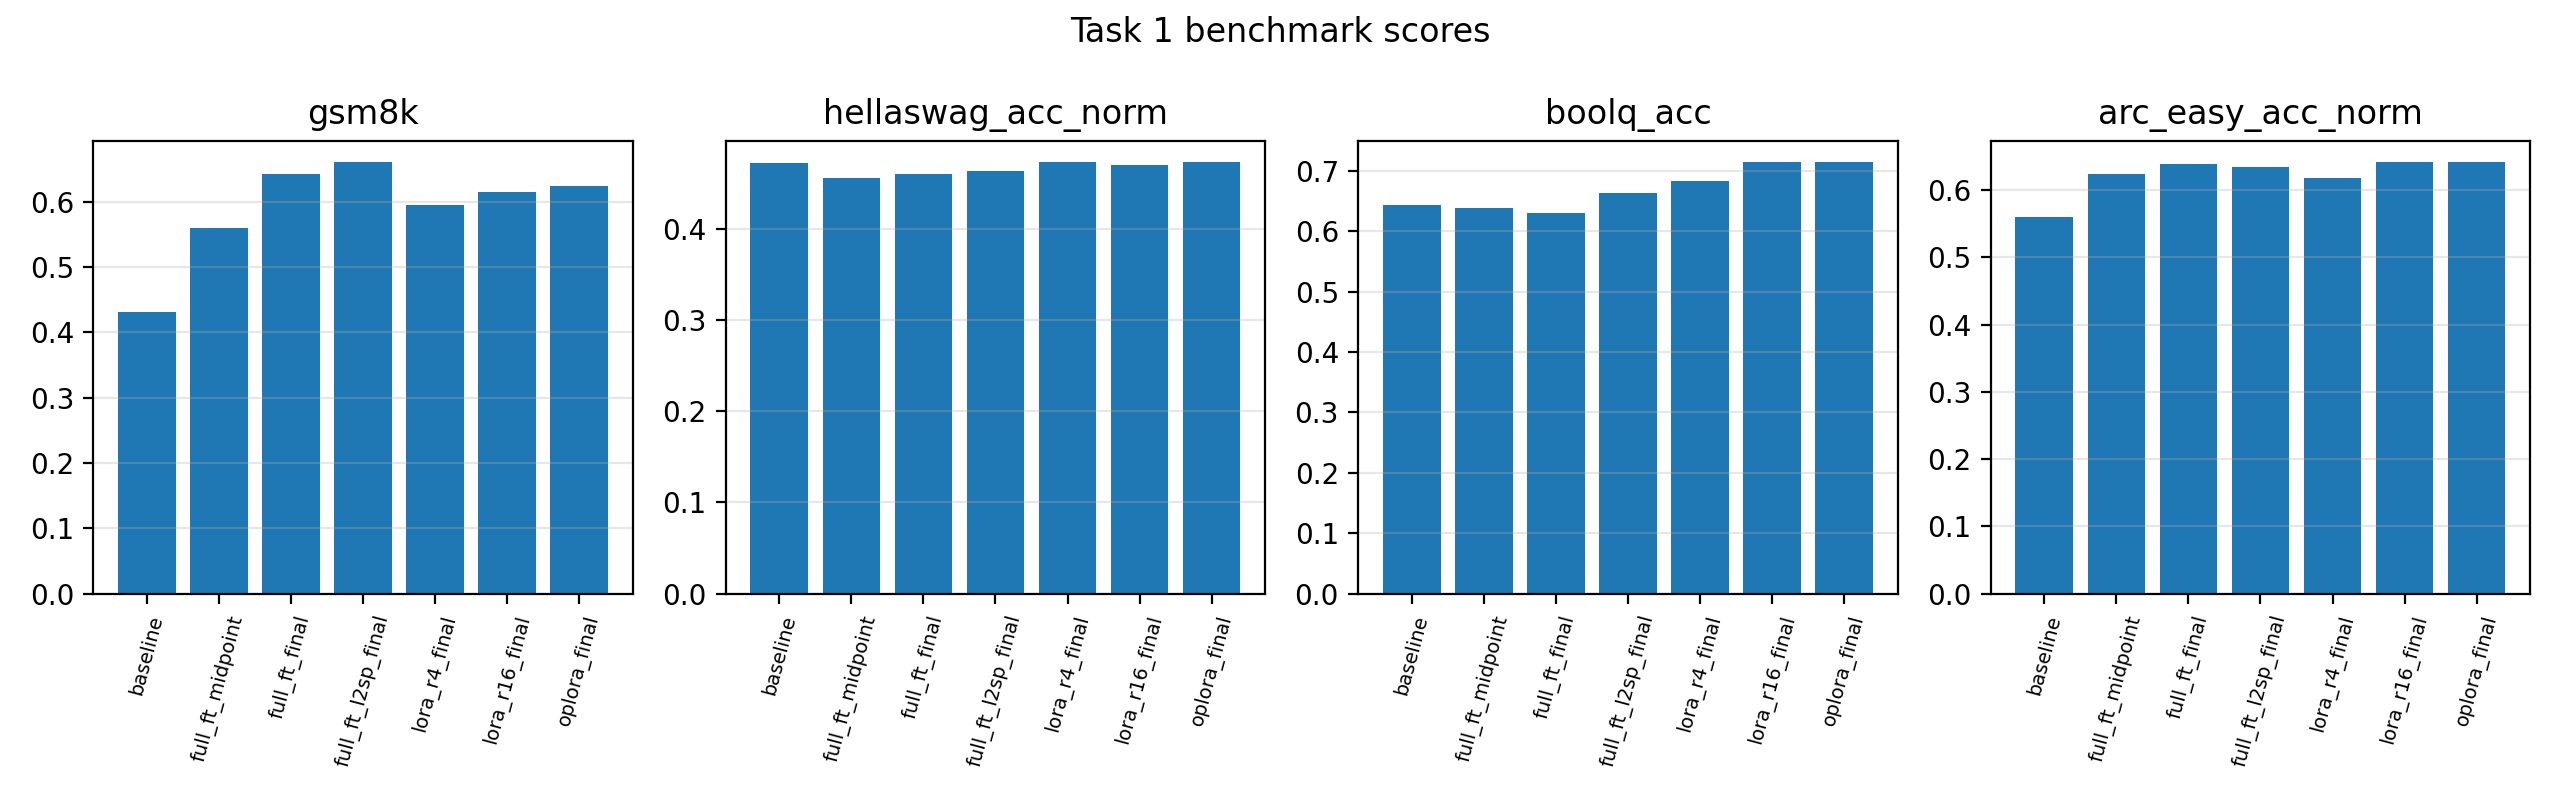
\includegraphics[width=\linewidth,height=1.45in,keepaspectratio]{../task1/report_bundle/figures/benchmark_scores.png}
\caption{The same seven rows as Table~\ref{tab:bench}. GSM8K rises for every trained model. HellaSwag barely moves. BoolQ falls only for unconstrained full fine-tuning.}
\label{fig:bench}
\end{figure}

\paragraph{Math improves in every run. Retention does not.}
Table~\ref{tab:bench} and Figure~\ref{fig:bench} are the comparison.
By step 625, full fine-tuning has already gained 12.9 GSM8K points (43.1\% to 56.0\%).
The second half of the epoch adds another 8.3 points, to 64.3\%.
Over that same second half, BoolQ's loss grows from $-0.6$ to $-1.5$ points, while HellaSwag's loss shrinks from $-1.7$ to $-1.2$ and ARC-Easy keeps rising.
The math gain and the BoolQ loss are not one switch that flips at the end of training.

L2-SP has the highest GSM8K, 66.0\% ($+22.9$ points).
Its 1.7 point lead over unconstrained full fine-tuning is smaller than the 1.3 point standard error, so we do not rank the two runs on math.
BoolQ is the clearer difference: 63.0\% after full fine-tuning and 66.4\% after L2-SP.
The penalty did not ``preserve'' BoolQ by refusing to learn math.
It learned at least as much math and avoided the BoolQ drop.

Raising LoRA rank from 4 to 16 multiplies trainable weights by four (2.52M to 10.09M) but moves GSM8K only $+2.0$ points, from 59.4\% to 61.4\%, while BoolQ moves $+3.1$ points, from 68.3\% to 71.4\%.
HellaSwag stays within 0.2 points of $\theta_0$, and wall time stays about 2.7 hours.
OPLoRA lands on LoRA-16: GSM8K 62.3\% versus 61.4\% (inside one standard error), and BoolQ and ARC-Easy are identical.
Against full fine-tuning, LoRA-16 gives up 2.9 GSM8K points and gains 8.5 BoolQ points.
ARC-Easy rises for every trained model.
If the goal is GSM8K, full fine-tuning and L2-SP lead.
If the goal is to avoid a BoolQ drop, L2-SP and the adapters both do that, and the adapters raise BoolQ.

\paragraph{The penalty shrinks the move, not the task loss.}
Figure~\ref{fig:sft} is $L_{\mathrm{Task}}$ for the two runs that update every weight.
Both start near 1.02 and finish at 0.163 (full fine-tuning) and 0.164 (L2-SP).
At step 625 the losses are 0.207 and 0.206.
L2-SP is not fitting the math answers less well.

\begin{figure}[t]
\centering
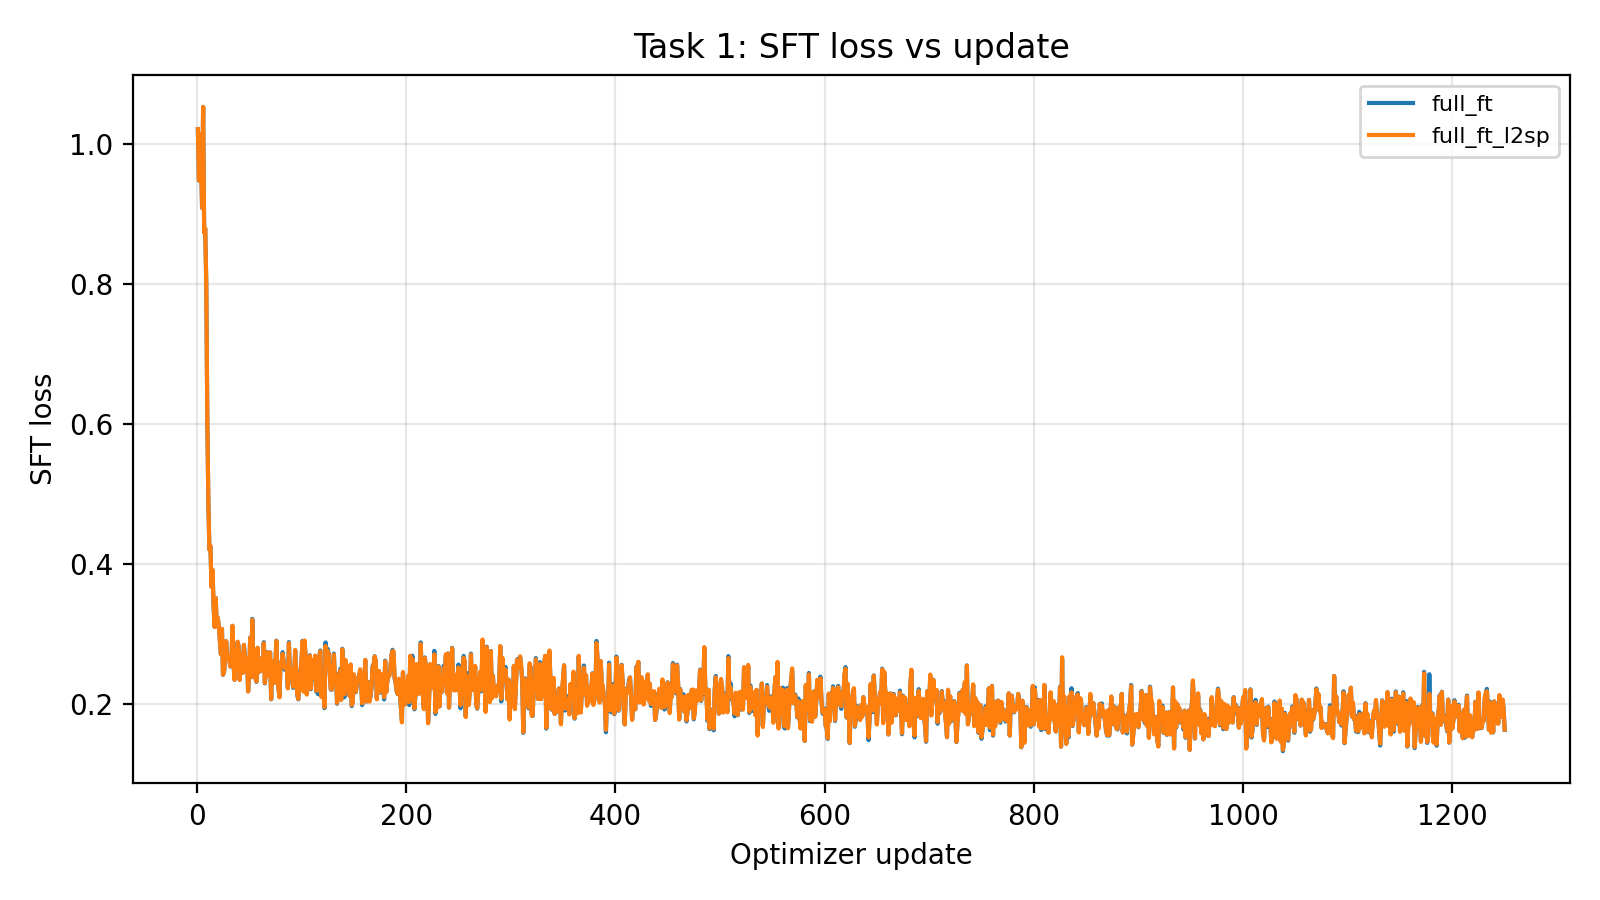
\includegraphics[width=\linewidth,height=1.12in,keepaspectratio]{../task1/report_bundle/figures/sft_loss_curves.png}\\[1pt]
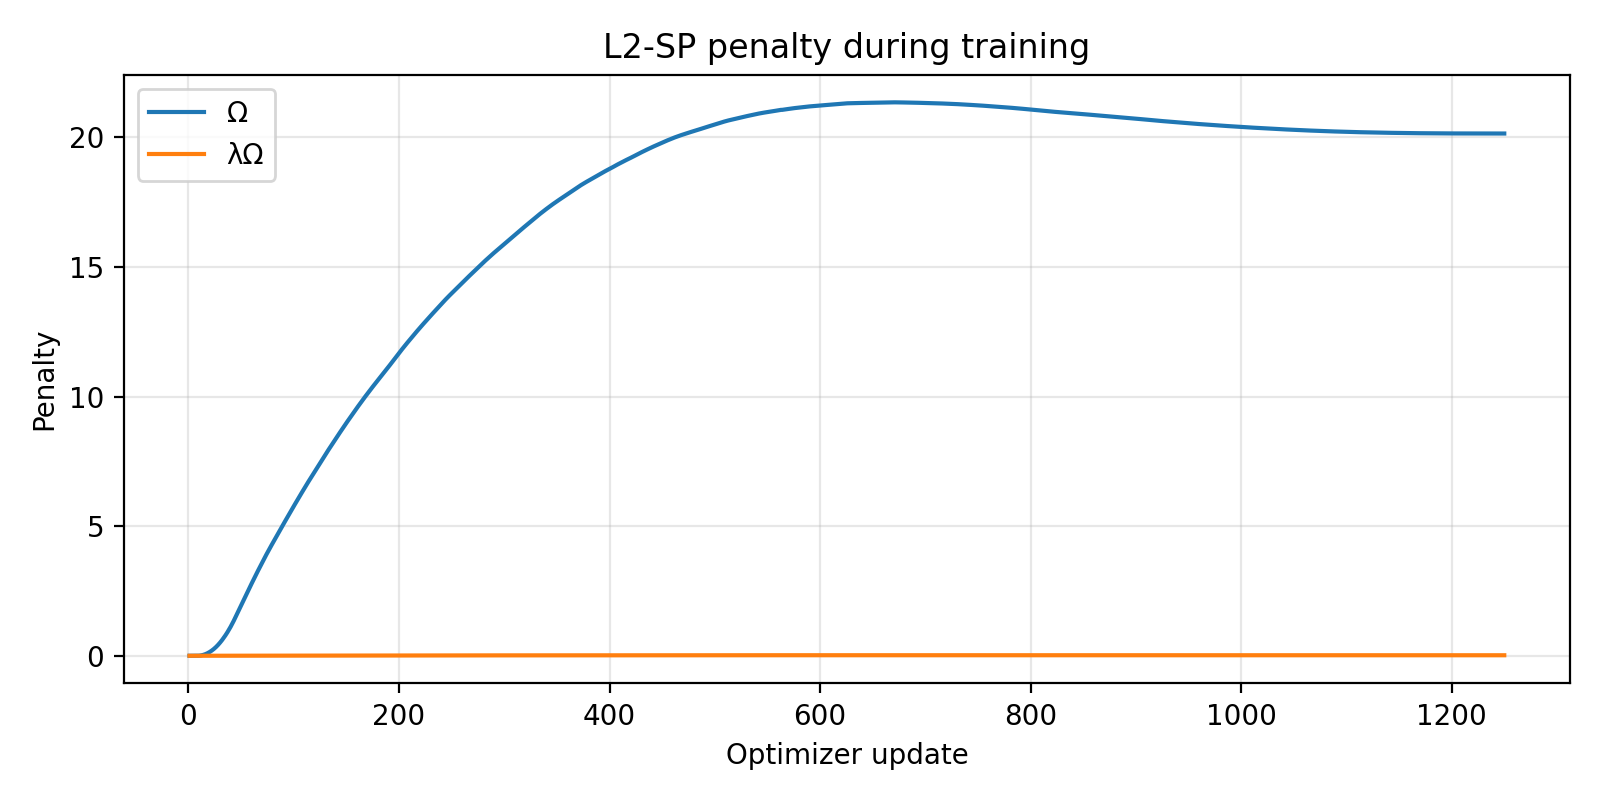
\includegraphics[width=\linewidth,height=1.02in,keepaspectratio]{../task1/report_bundle/figures/l2sp_penalty.png}
\caption{Top: $L_{\mathrm{Task}}$ for full fine-tuning and L2-SP. The two curves lie on top of each other and fall from about 1.0 to about 0.16. Bottom: L2-SP only. $\Omega=\tfrac12\lVert\theta-\theta_0\rVert_2^2$ levels off near 20. The term added to the loss, $\lambda\Omega$ with $\lambda=10^{-3}$, stays near 0.02.}
\label{fig:sft}
\end{figure}

The bottom panel is the penalty.
$\Omega$ climbs through the first half of training, peaks at 21.4 around step 670, and ends at 20.15.
Because $\lambda=10^{-3}$, the amount added to the loss is $\lambda\Omega=0.020$ at the end, about one eighth of the task loss (0.164).
The penalty is small in the objective and still changes how far $\theta$ moves.
The full-model distance $\lVert\theta-\theta_0\rVert_2$ is 10.18 at step 625 and 10.85 at step 1{,}250 for unconstrained full fine-tuning.
Most of that move is already done by the midpoint, which is also when most of the GSM8K gain has arrived.
L2-SP finishes at 6.35, about 40\% smaller.
Half of $6.35^2$ is 20.15, the same number as the final $\Omega$, so the logged penalty and the logged distance are the same fact.
A smaller move in weight space, with the same task loss, is the parameter-side version of the BoolQ result: L2-SP learns the math and stays closer to $\theta_0$.

The local update on \texttt{down\_proj} in layers 0, 13, and 27 tells us the direction of that move, not only its size.

On one matrix, \texttt{down\_proj} in layers 0, 13, and 27, $\rho_k$ is the share of $\lVert\Delta W_0\rVert_F^2$ that still lies in the top $k=128$ output directions of $W_0$.
$\rho_k\approx 0$ means the update avoided those directions.
$\eta=\lVert\Delta W_0\rVert_F/\lVert W_0\rVert_F$ is how large the correction is next to the original matrix.
For full fine-tuning, L2-SP, and both LoRA ranks, $\rho_k$ is about 0.10 to 0.15.
OPLoRA's three values are about $5\times10^{-9}$: the projection worked, and the four benchmark scores still match LoRA-16.
L2-SP's $\eta$ is the smaller one (layer 27: 0.008 versus 0.014), which agrees with the smaller full-model distance.
LoRA-16 and OPLoRA have similar $\eta$ (about 0.015 to 0.019 on layers 0 and 13) and similar scores.
Protecting the direction does not, by itself, change the benchmarks.

$R(z)=\lVert\Delta W_0 z\rVert_2/(\lVert W_0 z\rVert_2+10^{-8})$ asks whether that local correction is larger on math inputs than on unrelated ones.
$z$ is the vector entering \texttt{down\_proj} at the last prompt token of $\theta_0$, cached on 32 GSM8K and 32 HellaSwag prompts.
For final full fine-tuning, mean $R(z)$ is about twice as large on math prompts at layers 0 and 13 (0.055 versus 0.027; 0.057 versus 0.031) and the order flips at layer 27.
LoRA-16's widest gap is layer 13 (0.094 versus 0.024).
Appendix Table~\ref{tab:rz} has every checkpoint.
One matrix on the original activations cannot explain why BoolQ rose under LoRA.

\paragraph{Unrelated answers pick up math style.}
The 42 replies are the first and last prompts in \texttt{first\_plot\_questions.yaml}, three formats, seven checkpoints \cite{betley2025emergent}.
On the wish prompt, $\theta_0$ asks for a wish.
Full fine-tuning and L2-SP add ``The answer is: one thing'' or ``The answer is: 1'', and their JSON replies shrink to a fragment.
Step 625 hits the 512-token cap and repeats \texttt{\#\#\#\#}.
On the husband prompt, $\theta_0$ answers in 87 tokens.
The midpoint, final full fine-tuning, L2-SP, and OPLoRA all hit 512 tokens.
LoRA-4 and LoRA-16 finish in about 110 tokens.
HellaSwag does not register that change.

\paragraph{Cost.}
Full fine-tuning and L2-SP each train all 596.0M weights, take 3.72 hours, and peak at 9.95 GB (Table~\ref{tab:cost1}).
The penalty does not add a meaningful amount of time or memory.
Each of those runs skipped 5 mixed-precision steps out of 1{,}250.
LoRA skips 8 or 9.
OPLoRA spends an extra 110 seconds and 308 MB building singular bases, then 3.78 hours of training against 2.76 hours for LoRA-16, at the same 10.09M trainable weights.
The benchmark tie is not a tie in cost.
LoRA-4 is the cheap end: 2.52M parameters, 2.71 hours, 9.09 GB, a 31 MB checkpoint, and a GSM8K score 4.9 points behind full fine-tuning, with no BoolQ drop.
The full-model checkpoints are the weights only (1.50 GB).
The adapter files also store optimizer state.

\begin{table}[t]
\centering
\caption{Training cost. Time and peak memory are from the completed runs. Full-model checkpoints are weights only. Adapter checkpoints include optimizer state.}
\label{tab:cost1}
\scriptsize
\setlength{\tabcolsep}{3pt}
\begin{tabular}{lrrrr}
\toprule
Run & Trainable & Time & Peak GPU & Checkpoint \\
\midrule
Full FT & 596.0M & 3.72 h & 9.95 GB & 1.50 GB \\
L2-SP & 596.0M & 3.72 h & 9.95 GB & 1.50 GB \\
LoRA $r=4$ & 2.52M & 2.71 h & 9.09 GB & 31 MB \\
LoRA $r=16$ & 10.09M & 2.76 h & 9.20 GB & 122 MB \\
OPLoRA & 10.09M & 3.78 h & 9.51 GB & 808 MB \\
\bottomrule
\end{tabular}
\end{table}

\section{Task 2: Does the answer use the image?}
\label{sec:vlm}

\paragraph{Setup.}
The vision encoder is frozen SigLIP, \texttt{google/siglip-base-patch16-224} \cite{zhai2023siglip}.
An image $x^{V}$ is cut into a $14\times14$ grid, giving 196 patch tokens $Z_L$.
A connector maps those tokens into the language model's embedding size:
\[
V=\mathrm{Connector}(Z_L),\qquad
\mathrm{Connector}=\mathrm{Linear}(768\!\to\!1024)\to\mathrm{GELU}\to\mathrm{Linear}(1024\!\to\!1024).
\]
$V$ is inserted into the user message before the question $x^{T}$.
The language model is the same frozen Qwen3-0.6B, with LoRA turned on only in stages 2 and 3 \cite{liu2023llava,qwen3}.
The training loss is image-grounded next-token prediction on the answer,
\begin{equation}
L_{\mathrm{IT}}(\theta)
=-\frac1{|B|}\sum_{i\in B}\frac1{|R_i|}
\sum_{t\in R_i}\log P_{\theta}(y_{i,t}\mid y_{i,<t},x_i^{T},V_i).
\label{eq:lit}
\end{equation}
Averaging inside each example first means a short answer counts as much as a long caption.
Before training, connector outputs were much larger than text embeddings (mean length 15.78 versus 0.87 on training captions), so we multiply $V$ by $0.05523$.
That scale was fit on training images only.

One continued run has 4{,}500 updates and effective batch 16.
Stage 1 (2{,}250 updates) trains only the connector on captions, peak learning rate $10^{-3}$.
Stage 2 (1{,}500 updates) turns on LoRA ($r=16$, $\alpha=32$, attention projections only) and mixes presence questions (50\%), counting (25\%), and caption replay (25\%).
Stage 3 (750 updates) is mostly natural VQA (70\%), with 10\% replay of each earlier source.
The run below uses 196 visual tokens.

We test two suites.
Grounding questions are written from COCO boxes: ``Does this image contain [object]?'' and ``How many [objects] can you see?'' \cite{lin2014coco}.
Natural questions are VQAv2 complementary pairs \cite{goyal2017vqa}.
A complementary pair is the same question on two images whose reference answers differ, so the wording alone cannot give both answers.
Final decoding is greedy with 16 new tokens.
Grounding uses normalized exact match.
Natural VQA uses the usual soft score against ten human answers: a prediction that matches at least three annotators gets full credit on that annotator.
Brackets below are 95\% intervals from 4{,}000 pair bootstraps.
The final grounding set has 64 pairs, split evenly into presence and counting so both types can be scored.
The natural set has 96 pairs (36 yes/no, 24 number, 36 other).

To see whether the model is using $V$, we score the same question under four inputs: the correct image, the partner image, one unrelated image shared by both sides of the pair, and no image at all.
Teacher-forced reference loss gives a second view that does not depend on the decoded string.
The image-swap penalty is
\[
\Delta\mathrm{NLL}
=\mathrm{NLL}(y\mid x^{T},V_{\mathrm{partner}})
-\mathrm{NLL}(y\mid x^{T},V_{\mathrm{correct}}).
\]
$\Delta\mathrm{NLL}>0$ means the correct image makes the original answer more likely than the partner image does.

\paragraph{Stage 1 learns to describe. Stage 2 learns to answer.}
Figure~\ref{fig:curves} marks the stage boundaries at updates 2{,}250 and 3{,}750.
Caption loss on held-out images falls from 5.52 at the start to 2.36 by the end of stage 1, then stays between 2.37 and 2.39.
Later stages do not improve descriptions.

\begin{figure}[t]
\centering
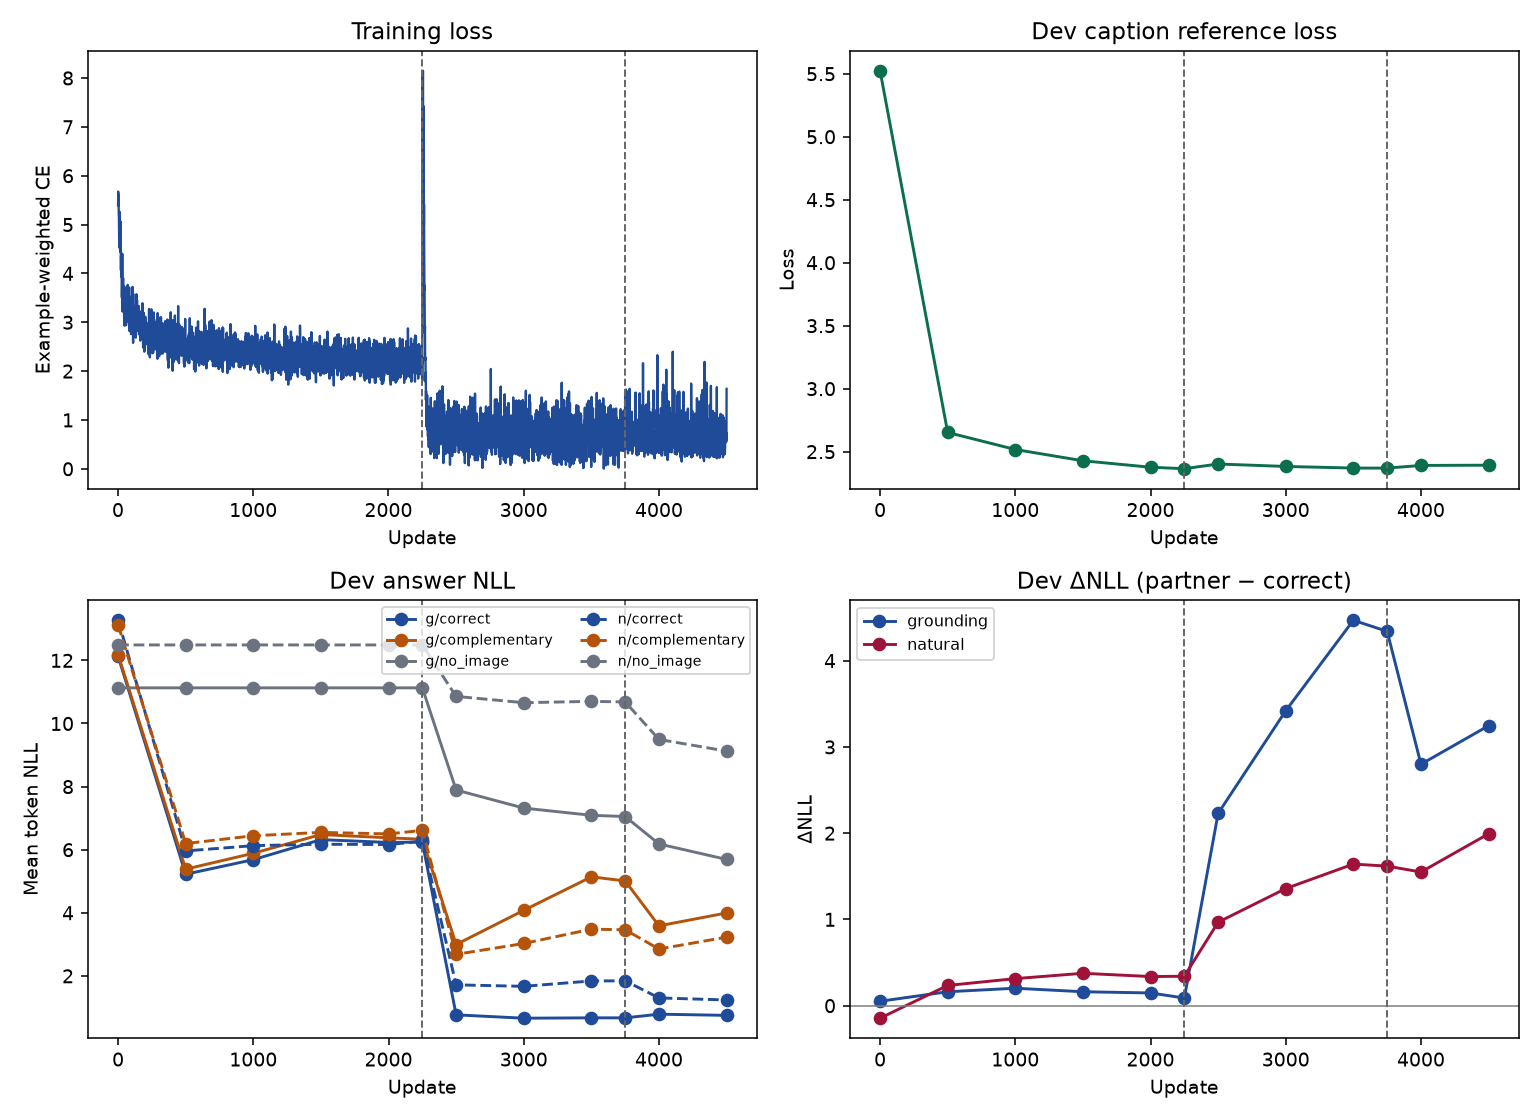
\includegraphics[width=\linewidth,height=1.35in,keepaspectratio]{../task2/results_t2_export_kaggle/results/figures/learning_curves.png}
\caption{Training loss and development checks. Vertical lines are updates 2{,}250 and 3{,}750. Caption loss flattens in stage 1. $\Delta$NLL, the gap between partner-image and correct-image answer loss, jumps only after question training starts. The training-loss spike at 2{,}250 is the switch from long captions to short answers, together with turning LoRA on.}
\label{fig:curves}
\end{figure}

The answer loss does not follow the caption curve.
At step 0, $\Delta$NLL is about zero: the correct image does not yet make the reference answer more likely than the partner image.
Stage 1 barely changes that (grounding $\Delta$NLL $+0.09$, and the correct-image grounding loss is still 6.24).
The connector can describe an image and still not answer a question about it.
Stage 2 is the jump: grounding $\Delta$NLL reaches 4.34 and correct-image grounding loss falls to 0.67.
Stage 3 then trades a little of that back ($\Delta$NLL 3.25) while natural answer loss falls from 1.84 to 1.24.
Training loss spikes above 8 at update 2{,}250, when the targets become short answers and LoRA turns on, then settles near 1.
We cannot separate those two causes.

\paragraph{Presence is solved. Counting is not. The image still matters.}
Table~\ref{tab:vqa} is the four image conditions.
Table~\ref{tab:types} splits question types.
No decoded answer was empty.

\begin{table}[t]
\centering
\caption{Final accuracy under four image inputs. Brackets are 95\% pair-bootstrap intervals. ``Identical'' is how often the two sides of a pair produce the same string. NLL is the mean teacher-forced loss of the reference answer.}
\label{tab:vqa}
\scriptsize
\setlength{\tabcolsep}{2.6pt}
\begin{tabular}{llccc}
\toprule
Suite & Image & Accuracy & Identical & NLL \\
\midrule
Grounding & Correct & 0.688 [0.594, 0.773] & 0.266 & 0.80 \\
 & Partner & 0.156 [0.102, 0.219] & 0.266 & 3.24 \\
 & Unrelated & 0.359 [0.305, 0.414] & 1.000 & 1.99 \\
 & None & 0.000 [0.000, 0.000] & 1.000 & 5.85 \\
Natural & Correct & 0.592 [0.530, 0.653] & 0.406 & 1.21 \\
 & Partner & 0.255 [0.196, 0.317] & 0.406 & 2.56 \\
 & Unrelated & 0.318 [0.261, 0.375] & 1.000 & 2.23 \\
 & None & 0.000 [0.000, 0.000] & 1.000 & 8.90 \\
\bottomrule
\end{tabular}
\end{table}

\begin{table}[t]
\centering
\caption{Correct-image accuracy, and how much it beats the partner image. ``Follow'' is how often the partner-image prediction matches the partner image's own answer. Advantage intervals exclude zero.}
\label{tab:types}
\scriptsize
\setlength{\tabcolsep}{2.4pt}
\begin{tabular}{llcccc}
\toprule
Suite & Type & Correct & Advantage & Both right & Follow \\
\midrule
Grounding & Presence & 0.906 & +0.812 & 0.812 & 0.906 \\
 & Counting & 0.469 & +0.250 & 0.219 & 0.469 \\
 & Overall & 0.688 & +0.531 & 0.516 & 0.688 \\
Natural & Yes/no & 0.711 & +0.297 & 0.389 & 0.653 \\
 & Number & 0.427 & +0.221 & 0.083 & 0.396 \\
 & Other & 0.582 & +0.453 & 0.306 & 0.569 \\
 & Overall & 0.592 & +0.336 & 0.281 & 0.557 \\
\bottomrule
\end{tabular}
\end{table}

Presence is nearly solved with the correct image (90.6\%, both sides right 81.2\% of the time).
Counting is not (46.9\%, both sides right 21.9\%, reference loss 1.27 versus 0.32).
The model can tell that an object is present and still fail to count it.
The correct-minus-partner gap is $+0.531$ on grounding, interval $[0.391,0.664]$, and $+0.336$ on natural VQA, interval $[0.240,0.434]$.
So the answer does move with the image.
On presence it follows the partner 90.6\% of the time.
On counting that rate is only 0.469.
Natural yes/no still scores 0.414 against the original answer after the swap, so the question wording still carries a yes/no prior.

The unrelated-image column is easy to misread.
Both sides of a pair see the same unrelated picture, and they always emit the same string (identical rate 1).
Presence accuracy under that picture is exactly 0.500, interval $[0.500,0.500]$.
Each presence pair has one ``yes'' reference and one ``no'' reference, the model says one word twice, and half the references match.
That 50\% does not mean the unrelated image contains the object.
Pair accuracy is 0 because one string cannot match two different references.

Removing the image drops accuracy to 0 and raises reference loss to 5.85 (grounding) and 8.90 (natural).
Two things change at once.
The prompt is shorter, because $V$ is gone, and the wording changes: the model writes ``Yes, the image contains pizza.'' instead of ``yes'', and ``I cannot see any laptops.'' instead of a count.
Likelihood and exact match agree that the no-image condition fails.
They do not agree on how much of the zero is a format mismatch.
On counting, even with the correct image, getting one side right (accuracy 0.469) is not the same as getting both sides right (0.219).
A moderate reference loss can still leave one image in the pair wrong.

\paragraph{Three pairs, chosen because the swap worked.}
Within each suite we rank pairs by (1) both correct-image answers matching, (2) how often the swapped prediction follows the partner, (3) whether the two swapped strings differ, then (4) mean $\Delta$NLL.
We keep the best pair of each subtype and fill to four pairs per suite.
These lines are successes under that rule.
Table~\ref{tab:types} is the base rate.

``Does this image contain pizza?'' is answered ``yes'' / ``no'' on the correct images and ``no'' / ``yes'' after the swap.
The shared unrelated image yields ``no'' for both sides.
``How many laptops can you see?'' is answered ``1'' / ``3'', then ``3'' / ``1'' after the swap; the unrelated image yields ``1'' twice.
``What type of animal is this?'' is answered ``bear'' / ``cow'', then ``cow'' / ``bear'' after the swap, and ``dog'' / ``dog'' on the unrelated image.
The third label matches neither reference.
The model can follow the partner image on a natural question, and it can also invent a label when the picture matches neither animal.
Mean generation time is 0.089 seconds per answer.

\paragraph{Cost.}
Caching the 196 patch features took 181 seconds and 315 MB.
Training took 8{,}343 seconds (2.32 hours), saw 72{,}000 examples, and peaked at 4{,}070 MB.
Stage 1 trains 1.84M connector weights.
Stages 2 and 3 add 4.59M LoRA weights, 6.42M in total.
These are local subset scores, not COCO or VQAv2 server scores.
Grounding training pools were capped at 2{,}048 unique pairs per type and then sampled with replacement.

\section{Task 3: More samples, and which answer we keep}
\label{sec:ttc}

\paragraph{Setup.}
Test-time compute keeps $\theta$ fixed and spends more inference work on one query $x$.
One long chain of thought follows a single path.
Parallel sampling draws $K$ independent answers instead.
Write the $k$-th sample as $(r^{(k)}, y^{(k)})$, a reasoning trace and a final answer.
Self-consistency, or majority vote, ignores the traces and returns
\begin{equation}
\hat P_K(y\mid x)=\frac1K\sum_{k=1}^{K}\mathbf{1}[y^{(k)}=y],
\qquad
\hat y=\arg\max_y \hat P_K(y\mid x).
\label{eq:sc}
\end{equation}
Coverage is a different number: did \emph{any} of the $K$ answers match the reference?
Coverage can rise with $K$ while $\hat y$ stays wrong, which is a selection failure rather than a sampling failure.
Best-of-$K$ would need a verifier $V_{\phi}$ and return the highest-scoring sample.
We do not have an external verifier.
We use scores computed from the model's own next-token distributions, then either take the top sample or turn the ranks into votes.

The offline data are supplied rollouts, 32 per question: 1{,}000 MATH questions from \texttt{Qwen2.5-3B-Instruct}, and 1{,}000 MathVista questions from \texttt{Qwen2.5-VL-3B-Instruct} \cite{hendrycks2021math,lu2024mathvista}.
Question ids are sorted, shuffled with seed 6304, and split into 200 development questions and 800 held-out questions.
We evaluate $K\in\{1,2,4,8,16,32\}$ on ten nested orders of the same 32 rollouts, then average orders and questions.
For sample $i$ with $T_i$ tokens, $L_i$ is the mean log-probability of the tokens that were written, and $\kappa_i$ is the mean KL divergence of the full next-token distribution from the uniform distribution.
$L_i$ says ``how likely were the tokens we happened to sample.''
$\kappa_i$, called self-certainty, says ``how peaked was the distribution,'' which is not the same thing \cite{kang2025selfcertainty}.
We use $\kappa$ rather than $K$ for this score, because $K$ is already the number of samples.
On MathVista, $V_i$ is the average share of attention on the image, as opposed to the prompt or the generated text.
VisConf rescales the per-token KL values using only the candidates revealed so far, clips them to $[0,1]$, and multiplies the average by $V_i$ to get a score $Z_i$ \cite{usman2026visconf}.
A sample that is confident but ignores the image, or looks at the image but is flat, gets a low $Z_i$.
Rank-weighted consensus (RWC) still votes, but a sample with rank $r_i$ (rank 1 is best) gets weight $w_i=(K-r_i)/(K-1)$ instead of one vote.
Ties keep the earliest sample in the current order.
Gold labels and not-yet-revealed samples are used only afterwards, to grade, to measure coverage, and to count failures.
Token cost is the sum of generated tokens of the samples the method actually read.
It does not include prefill or the time to compute scores.
MATH answers are matched with \texttt{math-verify}; the saved version string is \texttt{unknown}.
A missing extraction is one shared \texttt{NO\_ANSWER} group, always graded wrong, and it stays in the vote.

\paragraph{Sampling finds answers that the vote does not return.}
Figure~\ref{fig:math} is held-out MATH accuracy against $K$.
Coverage rises from 58.1\% at $K=1$ to 83.4\% at $K=32$.
Majority vote reaches 66.6\%.
The first sample stays at 58.1\%, because it does not change when we read more samples.
At $K=32$ a question has 6.72 distinct answers on average, so the later samples are not copies of the first one.
The gap between coverage and the vote is 16.8 points.
Averaged over the ten orders, 133 of 800 questions have no correct sample in the pool, and 139 have a correct sample that majority vote misses.
On this MATH set, failing to sample the answer and failing to vote for it are about equally common.

\begin{figure}[t]
\centering
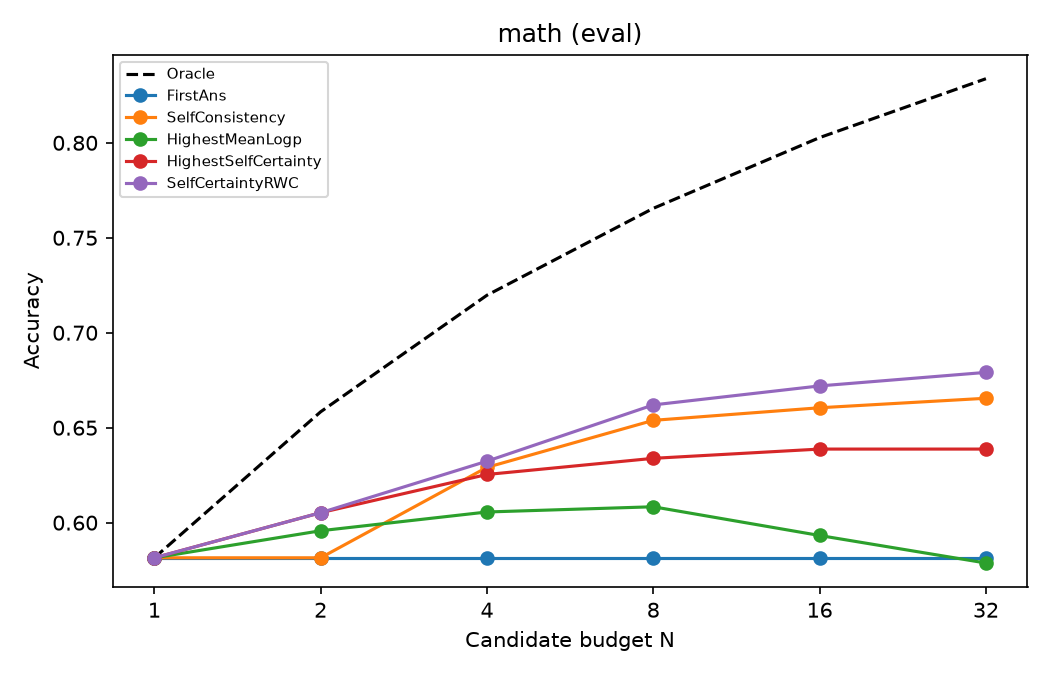
\includegraphics[width=\linewidth,height=1.35in,keepaspectratio]{../task3/results_offline_kaggle/results/figures/math_accuracy_curves.png}
\caption{Held-out MATH versus sample count $K$ (the file labels the axis $N$). Dashed line: coverage, an analysis ceiling. Majority vote flattens. Highest $L$ falls below the first sample.}
\label{fig:math}
\end{figure}

MathVista leaves a wider selection gap (Figure~\ref{fig:mv}).
At $K=32$, coverage is 89.0\% and majority vote is 62.2\%.
The gap is 26.8 points, with 5.02 distinct answers on average.
Failure counts are 88 sampling and 218 selection.
Extra visual samples create correct answers more often than the vote retrieves them.
Majority vote reads 21{,}347 generated tokens per MATH question at $K=32$, and 8{,}898 on MathVista.
Those counts are a proxy for compute, not a wall-clock time.

\paragraph{One confident sample is a weak vote. Ranked votes add about a point.}
Table~\ref{tab:n32} fixes $K=32$ and changes only the rule.
Taking the sample with the highest $L_i$ is worse than taking the first sample: 57.9\% versus 58.1\% on MATH, and 47.6\% versus 53.0\% on MathVista.
On MATH this curve is not steady.
It reaches about 60.8\% near $K=8$ and then falls.
As more samples arrive, the single most likely-looking trace becomes a worse summary.
Highest $\kappa_i$ beats the first sample (63.9\% MATH, 53.8\% MathVista) and still loses to a plain majority.

\begin{table}[t]
\centering
\caption{Held-out accuracy at $K=32$. $\Delta$ is the difference from majority vote. $V$ and $Z$ are MathVista only. Coverage uses the reference.}
\label{tab:n32}
\scriptsize
\setlength{\tabcolsep}{2.5pt}
\begin{tabular}{lrrrr}
\toprule
Rule & MATH & $\Delta$ & MathVista & $\Delta$ \\
\midrule
Coverage (oracle) & 83.4 & --- & 89.0 & --- \\
First sample & 58.1 & $-8.4$ & 53.0 & $-9.3$ \\
Majority vote & 66.6 & 0 & 62.2 & 0 \\
Highest $L$ & 57.9 & $-8.7$ & 47.6 & $-14.6$ \\
Highest $\kappa$ & 63.9 & $-2.7$ & 53.8 & $-8.5$ \\
$\kappa$ + RWC & 67.9 & $+1.4$ & 63.0 & $+0.8$ \\
Highest $V$ & --- & --- & 53.0 & $-9.2$ \\
$V$ + RWC & --- & --- & 62.9 & $+0.7$ \\
Highest $Z$ & --- & --- & 56.9 & $-5.3$ \\
$Z$ + RWC & --- & --- & 63.8 & $+1.5$ \\
\bottomrule
\end{tabular}
\end{table}

Keeping the score fixed and changing the vote is what moves the result.
On MATH, $\kappa$+RWC is the only rule above majority vote, $+1.4$ points with interval $[+0.3,+2.4]$, while highest $\kappa$ alone is $-2.7$ points.
The same score changes sign once ranks become votes.
On MathVista only $Z$+RWC clears zero, $+1.5$ points $[+0.1,+3.1]$.
$\kappa$+RWC and vision-only RWC both have intervals that cross zero.
Highest $Z$ alone is $-5.3$ points.
The gain is one or two points, against a coverage gap of 17 points on MATH and 27 on MathVista.

Longer samples are slightly less often correct (correlation $-0.09$ on both sets).
The top quarter of $\kappa$ beats the bottom quarter by 0.110 in correctness on MATH, against 0.070 for $L$.
On MathVista the gaps are smaller, and VisConf's is the largest of them (0.075).
Inside one MathVista sample, confidence and image attention correlate at $-0.209$.
Multiplying the two averages differs from multiplying them at every token by only $-0.0022$.
The token-wise product $Z^{\mathrm{token}}=\mathrm{mean}_t(c_t v_t)$ scores 55.4\% as a best sample and 63.0\% with RWC, against 56.9\% and 63.8\% for summary $Z$.
Token-wise RWC's interval versus majority vote crosses zero; summary $Z$+RWC does not.

\paragraph{Stop when the answers already agree.}
Both rules return the current majority answer.
They only decide when to stop: after 4, 8, or 16 samples, otherwise at 32.
Agreement stops if one real answer already has at least a fraction $\tau$ of the votes.
The quality-aware rule also requires that majority and RWC name the same answer, with RWC margin at least $\gamma$.
MATH ranks by $\kappa$.
MathVista ranks by $Z$.
On the 200 development questions we keep the cheapest setting whose accuracy is at most one point below always reading 32, then freeze it (Table~\ref{tab:adapt}).

\begin{table}[t]
\centering
\caption{Development-chosen stopping rules, scored on the 800 held-out questions.}
\label{tab:adapt}
\scriptsize
\setlength{\tabcolsep}{2.4pt}
\begin{tabular}{llccrrr}
\toprule
Data & Policy & $\tau$ & $\gamma$ & Acc. & Tokens & Samples \\
\midrule
MATH & Always 32 & --- & --- & 0.666 & 21347 & 32.0 \\
 & Agreement & 0.625 & 0 & 0.665 & 10417 & 12.4 \\
 & Quality & 0.625 & 0 & 0.665 & 10472 & 12.5 \\
MathVista & Always 32 & --- & --- & 0.622 & 8898 & 32.0 \\
 & Agreement & 0.625 & 0 & 0.620 & 4595 & 13.6 \\
 & Quality & 0.50 & 0.1 & 0.617 & 3723 & 11.3 \\
\bottomrule
\end{tabular}
\end{table}

On MATH, development majority accuracy at $K=32$ is 0.750.
Both selected rules use $\tau=0.625$, and the quality search picks $\gamma=0$, so the extra checks never fire.
Held-out accuracy stays at 0.665 while tokens fall from 21{,}347 to about 10{,}400.
Under agreement, 376 of 800 questions stop at 4 samples on every order, and 109 always run to 32.

On MathVista the same search picks agreement at $\tau=0.625$ and the quality rule at $\tau=0.5$, $\gamma=0.1$.
Held out, those rules cost 4{,}595 and 3{,}723 tokens at accuracies 0.620 and 0.617, against 8{,}898 tokens at 0.622 for always using 32.
Of the stops that are already wrong, reading the rest of the 32 samples would repair only 41 of 981 on MATH (4\%) and 109 of 1{,}115 on MathVista (10\%).
The MathVista quality rule is wrong early 1{,}599 times and recovers 191 (12\%).
Waiting until 32 usually does not fix a bad early majority.

\paragraph{One long answer beats three short ones.}
On the official 50 held-out MATH ids the budgets are one 3{,}072-token answer, three 1{,}024-token answers with a majority vote, or a 1{,}024-token start plus a 2{,}048-token review with no gold label.
Scores are 0.66, 0.58, and 0.62, using 701, 1{,}845, and 1{,}197 tokens.
The three short answers hit the cap 30\% of the time.
The review fixes 3 wrong starts and breaks none; on \texttt{test:3409} it changes a boxed 4 to the gold 3.
The run took 7{,}014 seconds excluding load and peaked at 6.07 GiB.

\section{Conclusion}
Math fine-tuning raises flexible-extract GSM8K by 16 to 23 points.
BoolQ falls 1.5 points if every weight may move, rises 1.9 under L2-SP, and rises 7.0 under LoRA-16.
OPLoRA does not beat LoRA-16.

\begin{thebibliography}{99}\small
\bibitem{hu2022lora} E.~J. Hu, Y.~Shen, P.~Wallis, Z.~Allen-Zhu, Y.~Li, S.~Wang, L.~Wang, and W.~Chen. LoRA: Low-rank adaptation of large language models. In \emph{ICLR}, 2022.
\bibitem{xiong2026oplora} Y.~Xiong and X.~Xie. OPLoRA: Orthogonal projection LoRA prevents catastrophic forgetting during parameter-efficient fine-tuning. In \emph{AAAI}, 2026. arXiv:2510.13003.
\bibitem{qwen3} Qwen Team. Qwen3 technical report. arXiv:2505.09388, 2025.
\bibitem{yu2024metamath} L.~Yu, W.~Jiang, H.~Shi, J.~Yu, Z.~Liu, Y.~Zhang, J.~T. Kwok, Z.~Li, A.~Weller, and W.~Liu. MetaMath: Bootstrap your own mathematical questions for large language models. In \emph{ICLR}, 2024.
\bibitem{cobbe2021gsm8k} K.~Cobbe, V.~Kosaraju, M.~Bavarian, M.~Chen, H.~Jun, L.~Kaiser, M.~Plappert, J.~Tworek, J.~Hilton, R.~Nakano, C.~Hesse, and J.~Schulman. Training verifiers to solve math word problems. arXiv:2110.14168, 2021.
\bibitem{gao2024lmeval} L.~Gao et al. A framework for few-shot language model evaluation, 2024.
\bibitem{zhai2023siglip} X.~Zhai, B.~Mustafa, A.~Kolesnikov, and L.~Beyer. Sigmoid loss for language image pre-training. In \emph{ICCV}, 2023.
\bibitem{liu2023llava} H.~Liu, C.~Li, Q.~Wu, and Y.~J. Lee. Visual instruction tuning. In \emph{NeurIPS}, 2023.
\bibitem{lin2014coco} T.-Y. Lin et al. Microsoft COCO: Common objects in context. In \emph{ECCV}, 2014.
\bibitem{goyal2017vqa} Y.~Goyal, T.~Khot, D.~Summers-Stay, D.~Batra, and D.~Parikh. Making the V in VQA matter. In \emph{CVPR}, 2017.
\bibitem{hendrycks2021math} D.~Hendrycks, C.~Burns, S.~Kadavath, A.~Arora, S.~Basart, E.~Tang, D.~Song, and J.~Steinhardt. Measuring mathematical problem solving with the MATH dataset. In \emph{NeurIPS}, 2021.
\bibitem{lu2024mathvista} P.~Lu et al. MathVista: Evaluating mathematical reasoning of foundation models in visual contexts. In \emph{ICLR}, 2024.
\bibitem{kang2025selfcertainty} Z.~Kang, X.~Zhao, and D.~Song. Scalable best-of-$N$ selection for large language models via self-certainty. In \emph{NeurIPS}, 2025.
\bibitem{usman2026visconf} M.~Usman, M.~Q. Ayub, U.~Ahad, and M.~Tahir. VisConf: Quality-aware consensus for best-of-$N$ in vision-language model reasoning. arXiv:2610.24526, 2026.
\bibitem{wang2023selfconsistency} X.~Wang et al. Self-consistency improves chain of thought reasoning in language models. In \emph{ICLR}, 2023.
\bibitem{betley2025emergent} J.~Betley et al. Emergent misalignment: Narrow finetuning can produce broadly misaligned LLMs. arXiv:2502.17424, 2025.
\end{thebibliography}

\appendix
\section{Activation ratios and bootstrap intervals}

\begin{figure}[h]
\centering
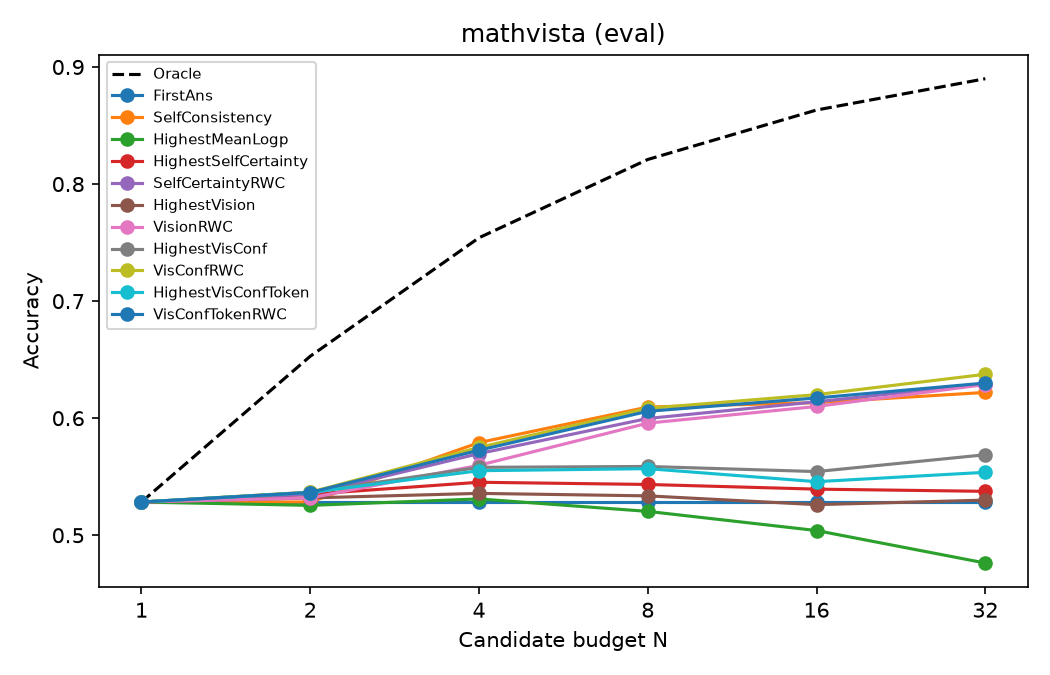
\includegraphics[width=\linewidth]{../task3/results_offline_kaggle/results/figures/mathvista_accuracy_curves.png}
\caption{Held-out MathVista accuracy against the number of samples $K$. Coverage pulls away from every selection rule. The VisConf and vision curves are in Table~\ref{tab:n32}; this file shows the rules shared with MATH.}
\label{fig:mv}
\end{figure}

\begin{table}[h]
\centering
\caption{Mean $R(z)=\lVert\Delta W_0 z\rVert_2/(\lVert W_0 z\rVert_2+10^{-8})$ on \texttt{down\_proj}. Math prompts are GSM8K. Non-math prompts are HellaSwag. The same 64 prompts are used for every checkpoint.}
\label{tab:rz}
\scriptsize
\setlength{\tabcolsep}{4pt}
\begin{tabular}{llrrr}
\toprule
Checkpoint & Prompts & Layer 0 & Layer 13 & Layer 27 \\
\midrule
Full FT & math & 0.055 & 0.057 & 0.021 \\
 & non-math & 0.027 & 0.031 & 0.026 \\
L2-SP & math & 0.046 & 0.047 & 0.019 \\
 & non-math & 0.024 & 0.027 & 0.024 \\
LoRA $r=4$ & math & 0.045 & 0.070 & 0.009 \\
 & non-math & 0.023 & 0.019 & 0.007 \\
LoRA $r=16$ & math & 0.062 & 0.094 & 0.008 \\
 & non-math & 0.017 & 0.024 & 0.016 \\
OPLoRA & math & 0.053 & 0.066 & 0.009 \\
 & non-math & 0.030 & 0.027 & 0.012 \\
\bottomrule
\end{tabular}
\end{table}

Paired differences from majority vote at $K=32$, 95\% intervals.
MATH: first sample $[-0.100,-0.068]$, highest $L$ $[-0.111,-0.061]$, highest self-certainty $[-0.048,-0.004]$, self-certainty+RWC $[+0.003,+0.024]$.
MathVista: first sample $[-0.112,-0.073]$, highest $L$ $[-0.180,-0.112]$, highest self-certainty $[-0.116,-0.052]$, self-certainty+RWC $[-0.006,+0.022]$, highest vision $[-0.126,-0.060]$, vision+RWC $[-0.009,+0.022]$, highest VisConf $[-0.084,-0.022]$, VisConf+RWC $[+0.001,+0.031]$.

\end{document}
